%%%%%%%%%%%%%%%%%%%%%%%%%%%%%%%%%%%%%%%%%%%%%%%%%%%%%%%%%%%%%%%%%%%
% Background
% Year:
% 2016、2017
% Team:
% Wolverine、RCPL
% Members: 
% Dexter Chen(Wolverine/2016), Eric Chang(Wolverine/2016), Eric Lee(Wolverine/2016), 
% Jacky Wu(Wolverine/2016), Karthick Mani(Wolverine/2016), Kenvin Lo(Wolverine/2016), 
% Yu-cheng Chen(Wolverine/2016), Paul Lin(RCPL/2017)
% (Format:Name(Team/Year))
% Relative files:
% Main.tex, Background_Information_retrieval_on_existing_database.tex, Library.bib, Wolverine_Background_Chart_1.png
% Note: 
% Do not compile this file compile Main.tex to get the pdf file instead.
%%%%%%%%%%%%%%%%%%%%%%%%%%%%%%%%%%%%%%%%%%%%%%%%%%%%%%%%%%%%%%%%%%%
	
\subsection{Information retrieval on existing database}
	We live in the time when technology develops rapidly. Information grows in an exponential rate. \cite{Tague1981} forecaster the further into the future we go, the fewer the additional number of first-rate publications. 
	Since the information increases from linear growth to exponential growth, we can't rely on the old ways to find the information we need. 
	Instead, we need new information retrieval methods to handle the big amount of data systematically. 
	
	However, most of the information retrieval methods such as search engine cannot search everything on the web. 
	\cite{Grehan2002} claimed a search engine which can only search the subset of the web it has ‘captured’ and included in its own database. 
	Therefore, we need to create a database to store these data and automatically update them.
	There are several online libraries currently available for us to get the academic articles or periodicals we need.
	Besides, they can be roughly divided into three groups according to the way they store articles based on the division used by National Taiwan University Library.\\

\paragraph{Index libraries:}
	These kind of libraries store the index and abstract of the articles.
	They don't provide the full-text documents directly, but they may provide the links to the publisher websites of articles.
	Besides, they can be categorized by the type of articles they include.
	
	\begin{itemize}		
		\item\textbf{Comprehensive topics}\\Libraries such as Web of Science, Scopus, Google Scholar...
		\item\textbf{Specialized topics}\\Libraries such as Compendex, BIOSIS Previews, PubMed, MEDline...		
	\end{itemize}
	
\paragraph{Publisher libraries:}
	These libraries are created by the publishers themselves, so they provide the newest and complete the documents directly.
	Besides, they can also be categorized by the type of articles they include.
	
	\begin{itemize}		
		\item\textbf{Comprehensive topics}\\Libraries such as Science Direct, Springer Link, Wiley Online Library...
		\item\textbf{Specialized topics}\\Libraries such as Nature.com, Emerald Management Xtra, IEEE Xplore...	
	\end{itemize}
	
\paragraph{Aggregator libraries:}
	These libraries do not publish the articles by themselves, but sometimes they still provide users with the full-text articles.
	The way they do this is to negotiate with some of the publisher libraries and get the authorization of the articles.
	Libraries such as EBSCOhost, ProQuest, JSTOR...

	The comparison between these libraries can be found on \textit figure \ref{WBC1}.
	On the next section we will discuss about more details about some of the existing libraries.

\begin{figure*}[htb]
	\begin{center}
		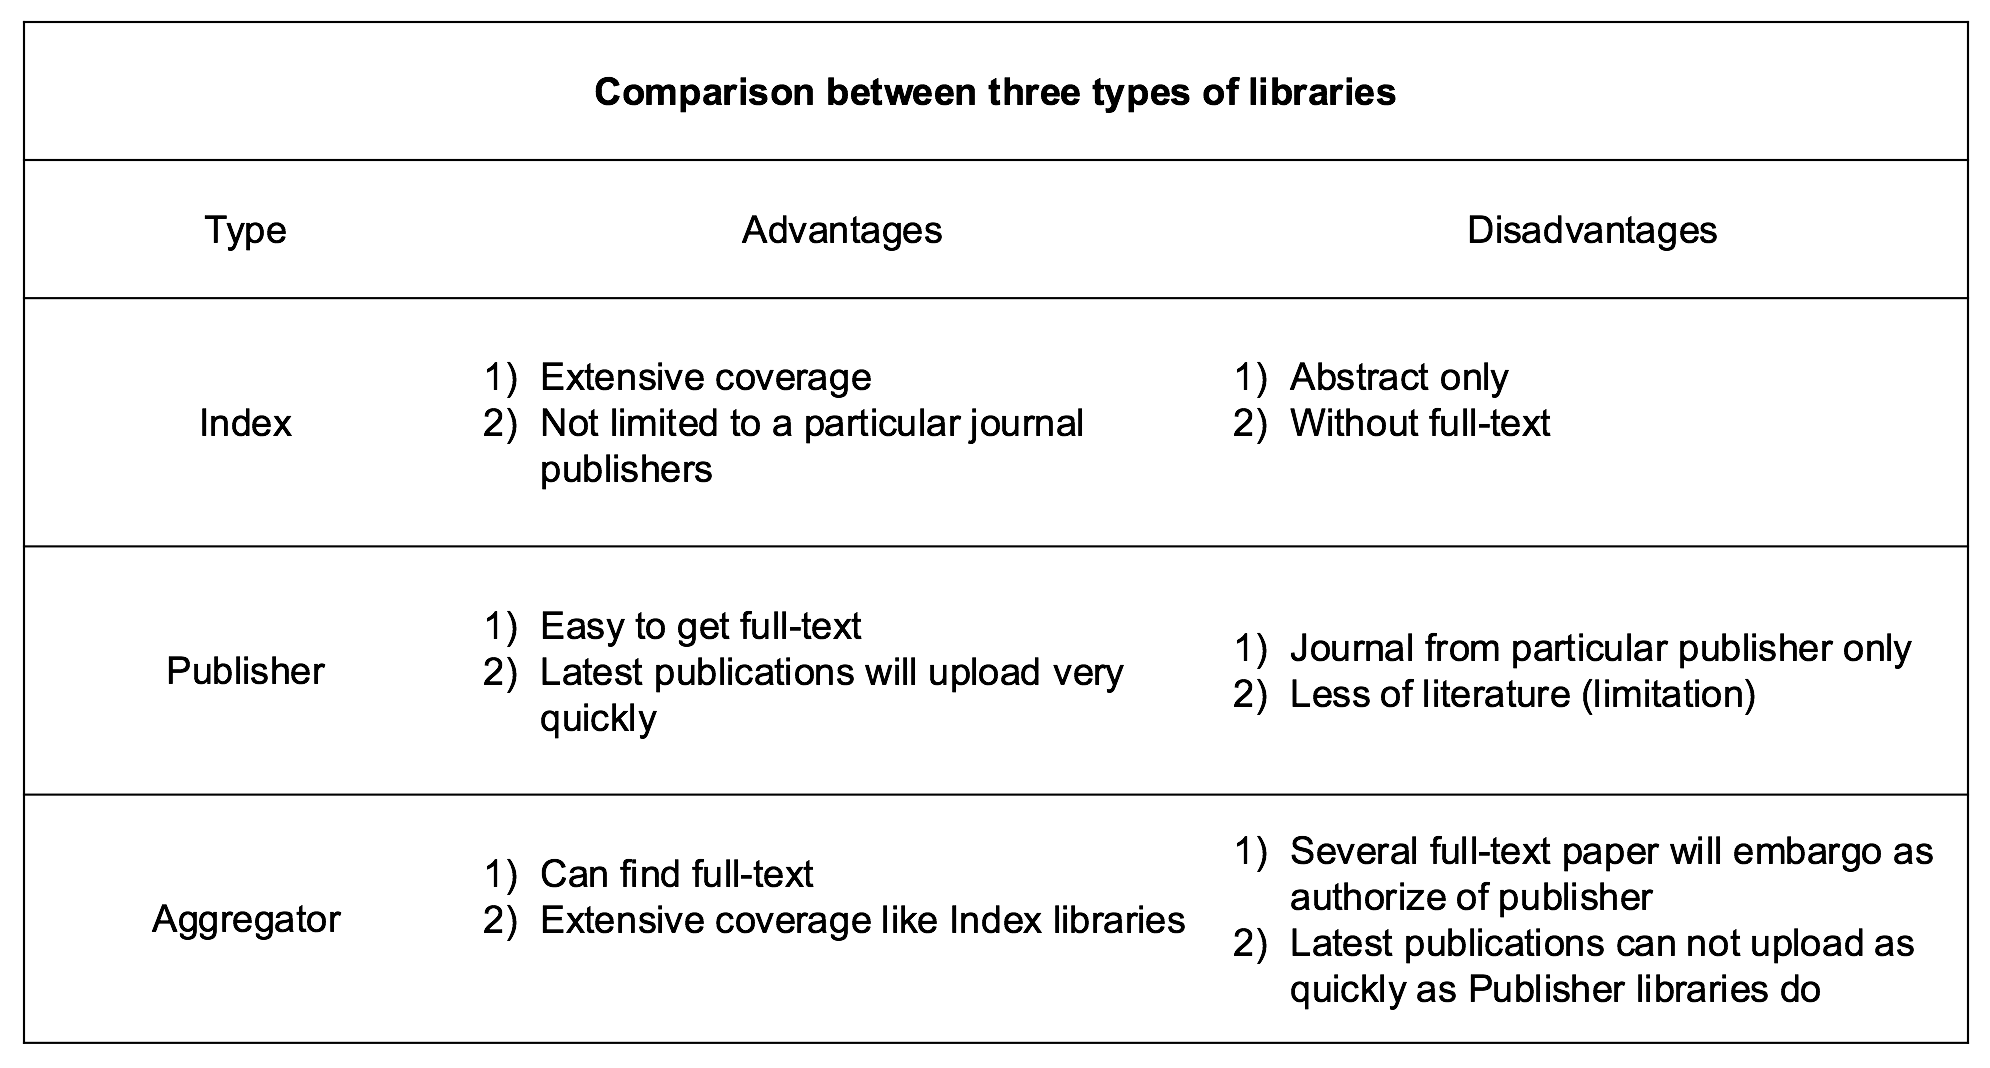
\includegraphics[width=0.8\textwidth]{Wolverine_Background_Chart_1}
	\end{center}
	\caption{Comparison between three types of libraries.\label{WBC1}}
\end{figure*}
\newpage

\subsubsection{Introduction to libraries }

\begin{enumerate}
	
	\item\textbf{PubMed}
	\setlength{\parindent}{1em}
	
	 PMC (PubMed Central) was launched in 2000.
	 PubMed citations often include links to the full-text article on the publishers' web sites or in PMC and the Bookshelf.
	 PubMed is a free library which is used for searching reference papers and abstracts related to the biomedical topics.
	 
	 The largest subset of PubMed is MEDLINE, which is a bibliographic database containing life sciences and biomedical information.
	 Both of them are built by National Library of Medicine. You may limit your search to MEDLINE only in PubMed.
	 A strong feature of PubMed is its ability to link MeSH(Medical Subject Headings) terms automatically. 
	 It is useful for people who want to find the medical articles.
	  
     Simple searches on PubMed can be carried out by entering the key words of a subject into PubMed's search window.
     PubMed translates this initial search formulation and automatically adds field names.
	 Like several libraries, people can find the specific result they desire by adding relevant MeSH terms, synonyms and Boolean operators.	 
	 The design philosophy of PubMed is based on full-text XML files, which are readable by machines, humans and moreover technology independent.
	 
	 PubMed is classified into Index libraries, which is the prime reason that it is not able to provide full text for some papers.
	 The type of database used by PubMed is Microsoft SQL server, which is a relational database to store all of the archives such as XML, images, and PDF files supplementary.
	
	\item\textbf{IEEE Xplore}
	\setlength{\parindent}{1em}	
	
	IEEE is an acronym for Institute of Electrical and Electronics Engineers, which is one of the leading standard organizations in the world. 
	Besides, it is one of the world's largest technical professional organization dedicated to advancing technology for the benefit of humanity. 
	There are more than 420,000 IEEE members in over 160 countries.
	And IEEE Xplore is a scholarly research library formerly known as IEEE/IET Electronic Library (IEL).
	
	The articles covered by IEEE Xplore are mainly from the IEEE and the Institution of Engineering and Technology(IET).
	More than 3.5-million full-text documents are in the field of electrical, engineering, computer science, and electronics are provided in this library. 
	There are many features in IEEE. It can rank the articles according to their click through rates or download times. 
    If some articles are updated by an author, those who set research alert on it will receive a notification through email by IEEE.
    However, some of the features are available for members only.
    Many enterprises and schools are the members of IEEE.
    
	
	\item\textbf{EBSCOhost}
	\setlength{\parindent}{1em}

	EBSCOhost is a popular reference which authorizes users to gain a great many full-text articles from proprietary databases.
	EBSCO Information Services, headquartered in Ipswich, Massachusetts, which is a division of EBSCO Industries Inc., the third largest private company in Birmingham, Alabama with annual sales of nearly $2$ billion according to the BBJ's 2013 Book of Lists.
    EBSCO offers library resources to customers in academic, medical, K–12, public library, law, corporate, and government markets. 
	Its products include EBSCONET, a complete e-resource management system, and EBSCOhost, which supplies a fee-based online research service with 375 full-text databases, a collectionof 600,000-plus ebooks, subject indexes, point-of-care medical references, and an array of historical digital archives.

    In 2010, EBSCO introduced its EBSCO Discovery Service (EDS) to institutions, which allows people to search a portfolio of journals and magazines

	\item\textbf{Google Scholar}
	\setlength{\parindent}{1em}
	
	Google Scholar is a freely accessible web search engine that indexes the full text or metadata of scholarly literature across an array of publishing formats and disciplines. Released in beta in November 2004, the Google Scholar index includes most peer-reviewed online academic journals and books, conference papers, theses and dissertations, preprints, abstracts, technical reports, and other scholarly literature, including court opinions and patents. While Google does not publish the size of Google Scholar's database, third-party researchers estimated it to contain roughly 160 million documents as of May 2014 and an earlier statistical estimate published in PLOS ONE using a Mark and recapture method estimated approximately $80-90$ coverage of all articles published in English with an estimate of 100 million. This estimate also determined how many documents were freely available on the web.
	
	Google Scholar is similar in function to the freely available CiteSeerX and getCITED. It also resembles the subscription-based tools, Elsevier's Scopus and Thomson Reuters' Web of Science.
		
	For further references see \href{https://en.wikipedia.org/wiki/Google_Scholar}{Google-Scholar Wiki}
	
	\item\textbf{Comparison of PubMed, Scopus, Web of Science, and Google Scholar: strengths and weaknesses}
	\setlength{\parindent}{1em}
	
	PubMed, Google Scholar, and Web of Science originate from the United States, whereas Scopus originates from Europe. PubMed and Google Scholar are free and
	provide open access to all interested clinicians, researchers, and trainees and also to the public in general. Scopus and Web of Science are databases that
	belong to commercial providers and require an access fee. Regarding Google Scholar, although relevant data are not summarized anywhere, the database is essentially a part of a popular WWW search engine, which means that there are no limits on the languages covered, keywords allowed per search, and list of covered journals, provided for the latter that an electronic edition exists. Similarly there are no data for the frequency of Google Scholar updates (see later discussion of this topic).
		
	PubMed focuses mainly on medicine and biomedical sciences, whereas Scopus, Web of Science, and Google Scholar cover most scientific fields. Web of Science
	covers the oldest publications, because its indexed and archived records go back to 1900. PubMed allows the larger number of keywords per search but is the only database of the four that does not provide citation analysis. Scopus includes articles published from 1966 on, but information regarding citation analysis is available only for articles published after 1996.
	
	PubMed was developed by the NLM, a division of the National Institutes of Health, and rapidly became synonymous with medical literature research worldwide. It 	offers a quick free search with numerous keywords as well as limited searching with various criteria [i.e., search by authors, journal, date of publication, date of addition to PubMed, or type of article]. The results of	a search can be displayed in a listing including from 5–500 items per page or as a summary [in which the full title, the names of the authors, the source and PubMed identification (PMID) of each article are presented],
	and the list can also be presented with abstracts, if available. Information on whether an abstract is available, and free text access is comprehensively represented by a displayed icon. A search can easily be sent to text, a file, the clipboard, e-mail, an RSS feed, and an 	order. PubMed also allows for direct use of other search engines developed by the NLM, such as GENSAT,
	OMIM, and PMC, the latter allowing for free full text access to a wide array of previous decades’ publications from numerous journals. Thus, PubMed now offers larger than one million freely available articles of which a significant
	number come from digitized back issues.
	
	One major advantage of PubMed, not reproduced by Scopus or Web of Science, is that it is readily updated 	not only with printed literature but also with literature 	that has been presented online in an early version before print publication by various journals. In contrast, Scopus and Web of Science are readily updated for printed literature but do not include online early
	versions.
	
	The Scopus database was developed by Elsevier, combining the characteristics of both PubMed and Web of Science. These combined characteristics allow
	for enhanced utility, both for medical literature research and academic needs (citation analysis), yet access to the database is not free, although reviewers for numerous Elsevier medical journals are entitled to 1 month of free use. It offers a quick search, a basic search, an author search, an advanced search, and a source search. In the basic search the results for the keywords chosen can be limited by date of publishing, by addition to Scopus, by document type, and by subject areas, whereas the author search is based only on author names. The advanced search combines the basic search without the limits and the author search, and more operators and codes are allowed. The source search is confined to selection of a subject area, a source type (i.e., trade publication or conference proceedings), a source title, the ISSN number, and the publisher.
	
	The search results in Scopus can be displayed as a listing of 20–200 items per page, and documents can be saved to a list and/or can be exported, printed, or
	e-mailed. The results can be refined by source title, author name, year of publication, document type, and/or subject area, and a new search can be initiated within the results. The presence of an abstract, references, and free full text is noted under each article title, in addition to where these can be found. When abstracts are displayed, the keywords are highlighted. The fields that can be included in the output are optional (i.e., citation information, bibliographical information,abstract, and keywords). The citation analysis that Scopus performs is presented as a table with numbers of cited articles for individual years, as well as the total number of cited references for all years. The articles cited can be accessed by simply clicking on the number of citations. In addition, Scopus has search tips written in 10 languages. 
	
	Web of Science was developed by Thomson Scientific, a part of the Thomson Corporation, another private company, and has dominated the field of academic reference, mainly through the annual release of the journal impact factor, a tool for evaluating the importance and influence of specific publications. The impact factor has been highly criticized but remains the most widely used of the indexes available. It has a quick search (by entering a topic), an advanced search, a general search, and a cited reference search. Help is offered for all types of searches of author, of group author, and of full source title, as well as of abbreviations. In the cited reference search the search can be limited by cited author, cited work, and cited years, whereas the cited author index and the cited work index can be presented, if the researcher requires it. The results of a search can be displayed as a listing of 10–50 items per page. The full title, author names, and source are provided. When the full text is available, the option of “view free full text” is present. Related records
	can be found, sorted by latest date, times cited, relevance, first author, publication year, and source title. The results can be analyzed (i.e., by author, country/territory, or document type), and the citation report is
	presented with a label bar chart. The results can be refined, and the researcher can view or exclude records.
	
	Google Scholar was developed by Google Inc., another private company, but it is freely accessible and aims to summarize all electronic references on a subject. There is no journal frame/list available for Google Scholar, because it presumably lists all publications that 	have emerged from the electronic search. Being essentially a Web search engine, its aim is to reach the widest
	audience available. It allows a quick search and an advanced search. In the advanced search the results can be limited by title words, authors, source, date of publication, and subject areas. The languages of the interface and of the search are optional. The results can be displayed as a listing of 10–300 items per page. Each retrieved article is represented by title, authors, and
	source, but the abstract and information on free full text availability are not provided by Google Scholar. Under each retrieved article the number of cited
	articles is noted and can be retrieved by clicking on the relevant link. By clicking on the article title, Google Scholar leads you to a list of possible links to the article, usually on the journal’s site, but for older articles the
	link is directed to the PubMed citation. In addition, Google Scholar provides links to relevant articles and 	allows for a general Google Web search, using selfselected keywords from the article and the author name.
	
	For more detail see \cite{Matthew2008}
\end{enumerate}

